\documentclass[12pt,a4paper,oneside]{article}
\usepackage[utf8]{inputenc}
\usepackage[czech]{babel}
\usepackage[T1]{fontenc}
\usepackage{amsmath}
\usepackage{amsfonts}
\usepackage{amssymb}
\usepackage{graphicx}
\usepackage{intcalc}
\usepackage{caption}
\usepackage{subcaption}

\usepackage{float}
\usepackage{enumitem}

\newcommand*{\Myitem}{% 
   \item[{\includegraphics[width=.5cm]{images/type\intcalcMod{\value{enumi}}{11}.png}}]\stepcounter{enumi}% 
}

\newcommand*{\Treeitem}{% 
   \item[{\includegraphics[width=.65cm]{images/tree\intcalcMod{\value{enumi}}{18}.png}}]\stepcounter{enumi}% 
}

\newcommand*{\Treemenu}{% 
   \item[{\includegraphics[width=.65cm]{images/treemenu\intcalcMod{\value{enumi}}{3}.png}}]\stepcounter{enumi}% 
}

\newcommand*{\Mapmenu}{% 
   \item[{\includegraphics[width=.65cm]{images/mapmenu\intcalcMod{\value{enumi}}{8}.png}}]\stepcounter{enumi}% 
}


\begin{document}
%%%%%%%%%%%%%%%%%%%%%%%%%%%%%%%%%%%%%%%%%%%%%%%%%%%%%%%%%%%%%%%%%%%%%%%%%%%%%%%%%%%%%%%%%%%%%%%%%%%%%%%%%%%%%%%%%%%%%%%%%%%%%%%%
	\begin{titlepage}	
		\begin{center}
		 	\null
			\vfil
			{\fontsize{70}{60}\selectfont \textbf{DeskChar}}
			
			
			\vspace{0.4cm}
			{\fontsize{15}{40}\selectfont
				Uživatelská příručka pro hráče a Pána jeskyně
			}
			\vfil			
			\includegraphics[width=6cm]{images/char}
			
			\vspace{8 cm}
			{\fontsize{20}{40}\selectfont
				Jan Horáček				
			}

			

		\end{center}
	\end{titlepage}
%%%%%%%%%%%%%%%%%%%%%%%%%%%%%%%%%%%%%%%%%%%%%%%%%%%%%%%%%%%%%%%%%%%%%%%%%%%%%%%%%%%%%%%%%%%%%%%%%%%%%%%%%%%%%%%%%%%%%%%%%%%%%%%%

	\setcounter{page}{1}
	\tableofcontents
	\newpage
	
%%%%%%%%%%%%%%%%%%%%%%%%%%%%%%%%%%%%%%%%%%%%%%%%%%%%%%%%%%%%%%%%%%%%%%%%%%%%%%%%%%%%%%%%%%%%%%%%%%%%%%%%%%%%%%%%%%%%%%%%%%%%%%%%

	\section{Úvod}
Aplikace DeskChar byla vytvořena za účelem doplnění mobilní aplikace MobChar, která slouží jako osobní deník pro hráče a také jako řídící aplikace pro Pána jeskyně pro hry na hrdiny jako jsou Dračí doupě, Dungeons\&dragons a další. Aplikaci je možné spustit na operačních systémech Windows a Linux, pro každý operační systém existuje program. \par

Tato příručka se týká užívání aplikace DeskChar.

		\vspace{1cm}		
		
Aplikace DeskChar umožňuje dvě základní funkcionality. Mobilní aplikace DeskChar pro Dračí doupě využívají systém šablon. Tyto šablon se využívají pro vytváření všech objektů v mobilní aplikaci. Šablony je možné do aplikace importovat pomocí XML souboru. Tyto XML soubory je možné v aplikaci vytvářet. \par

Druhá hlavní funkcionalita aplikace se týká vytváření celého dobrodružství. Lze vytvářet lokace, příšery, předměty, mapy a další potřebné objekty pro tvorbu dobrodružství. Vytvořené dobrodružství je možné vyexportovat do strukturovaného XML souboru, které se dá následně importovat do mobilní aplikace MobChar pro balíček Pána jekyně. Další možnost je exportovat dobrodružství do přehledného HTML formátu, který je uzpůsobený pro tisk, což bude vyhovovat převážně Pánům jeskyně, kteří nechtějí využívat při hraní mobilní telefony. Šablony je samozřejmě také možné z mobilních aplikací importovat a dále na nich pracovat. 
		\newpage

%%%%%%%%%%%%%%%%%%%%%%%%%%%%%%%%%%%%%%%%%%%%%%%%%%%%%%%%%%%%%%%%%%%%%%%%%%%%%%%%%%%%%%%%%%%%%%%%%%%%%%%%%%%%%%%%%%%%%%%%%%%%%%%%

	\section{První spuštění aplikace}
Při prvním spuštění aplikace otevře prázdné okno pouze se základními ovládacími prvky [\ref{fig:first_run}]. Aplikace při každém spuštění neobsahuje žádná data, protože databáze běží pouze v paměti. Pokud chcete pracovat ve své předchozí práci, je nutné nejdříve otevřít soubor s daty. 		
%	\vfill
				
	\begin{figure}[h]
  		\centering
  		\begin{minipage}[t]{0.8\textwidth}
    		\includegraphics[width=\linewidth]{images/first_run}
    		\caption{Obrazovka programu při prvním spuštění}
    		\label{fig:first_run}
  		\end{minipage}
  		
	\end{figure}
	
	\newpage
	
%%%%%%%%%%%%%%%%%%%%%%%%%%%%%%%%%%%%%%%%%%%%%%%%%%%%%%%%%%%%%%%%%%%%%%%%%%%%%%%%%%%%%%%%%%%%%%%%%%%%%%%%%%%%%%%%%%%%%%%%%%%%%%%%

	\section{Hlavní menu}
Hlavní menu aplikace je členěno na tři části, \texttt{Soubor} kde se nacházejí základní operace s aplikací a souborem drd. Menu \texttt{Šablony} obsahuje možnosti, pro vybrání editace cílových šablon. Poslední menu \texttt{Nápověda} obsahuje pouze položku \texttt{O aplikaci}. \par
			
	\begin{figure}[h]
  		\centering
  		\begin{minipage}[t]{0.48\textwidth}
    		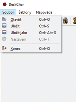
\includegraphics[width=\linewidth]{images/menu_soubor.png}
    		\caption{Menu pro základní operace}
    		\label{fig:menu_soubor}
  		\end{minipage}
  		\hfill
  		\begin{minipage}[t]{0.48\textwidth}
  			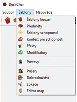
\includegraphics[width=\linewidth]{images/menu_sablony.png}
    		\caption{Menu pro zvoleni šablony}
    		\label{fig:menu_sablony}
  		\end{minipage}
	\end{figure}
	
	\subsection{Menu soubor}
	V menu soubor se nacházejí možnosti převážně pro práci s celým programem. 
	\begin{description}
		\item[Otevřít (Ctrl+O)] Položka otevřít slouží k otevření souboru s koncovkou .drd, ve které se nachází uložené dobrodružství. Po zvolení možnosti se otevře dialog pro zvolení souboru s koncovkou .drd. Po zvolení souboru dvojklikem, nebo vybárním souboru a potvrzení možností otevřít, se data obsažené v souboru nahrají do aplikace a otevře se záložka Dobrodružství.
		
		\item[Uložit (Ctrl+S)]
{description} Položka uložit slouží pro uložení stávajícího stavu aplikace do souboru s koncovkou .drd. Pokud v aplikaci byl otevřen soubor .drd, po zvolení možnosti uložit se stávají stav aplikace uloží do stejného souboru, ze kterého byl otevřen. Pokud již bylo dobrodružství uloženo do konkrétního souboru, aktuální stav se automaticky uloží do tohoto souboru. Pokud ani jedna z těchto možností se nestala, volba uložit se zachová stejně jako možnost Uložit jako
	
		\item[Uložit jako (Ctrl+Alt+S)] Položka jako slouží pro uložení stávajícího stavu aplikace do souboru. Od položky uložit se liší tím, že se vždy zeptá na cílové umístění. Po zvolení cílového souboru, se stav aplikace uloží do zvoleného souboru. 
		
		\item[Nastavení (Ctrl+T)] Položka nastavení otevře nové okno s nastavením. Podrobnější popis nastavení se nachází dále.
		
		\item[Konec (Ctrl+Q)] Položka konec slouží k ukončení aplikace. Před ukončením aplikace je uživatel dotázán, zda si přeje aktuální stav aplikace uložit
		
	\end{description}
	
	\subsection{Menu šablony}
	V menu šablony se nachází možnosti, kterými zvolíte konkrétní editační záložku šablon nebo objektů. Zvolením položky se přepnete do editace konkrétních šablon a objektů.
	
	\begin{description}
		\item[Kouzla] Editace šablon kouzle
		\item[Předměty] Editace šablon předmětů
		\item[Schopnosti] Editace šablon schopností
		\item[Kontext pro schopností] Editace šablon pro kontext schopností
		\item[Efekty] Editace šablon efektů
		\item[Modifikátory] Editace šablon modifikátorů
		\item[Postavy] Editace postav
		\item[Příšery] Editace šablon příšer
		\item[Dobrodružství] Editace dobrodružství
		\item[Lokace] Editace šablon lokací
		\item[Map] Editace map
	\end{description}
%%%%%%%%%%%%%%%%%%%%%%%%%%%%%%%%%%%%%%%%%%%%%%%%%%%%%%%%%%%%%%%%%%%%%%%%%%%%%%%%%%%%%%%%%%%%%%%%%%%%%%%%%%%%%%%%%%%%%%%%%%%%%%%%

	\section{Hlavní toolbar}
Na hlavní obrazovce se nachází toolbar, pomocí kterého se dá snadno přepínat mezi druhy šablon. Toolbar je na obrázku \ref{fig:toolbar}. Každá ikona otevře konkrétní editace objektů.
	
	\begin{figure}[h]
  		\centering
  		\begin{minipage}[t]{1\textwidth}
    		\includegraphics[width=\linewidth]{images/toolbar}
    		\caption{Toolbar se základními šablonami}
    		\label{fig:toolbar}
  		\end{minipage}
  		
  		\vfill
	\end{figure}
	
\begin{enumerate}[leftmargin=2cm]
   \Myitem Editace kouzel.
   \Myitem Editace předmětů.
   \Myitem Editace schopností.
   \Myitem Editace kontextu schopností.
   \Myitem Editace efektů.
   \Myitem Editace modifikátorů.
   \Myitem Editace postav.
   \Myitem Editace příšer.
   \Myitem Editace dobrodružství.
   \Myitem Editace lokací.
   \Myitem Editace map.
\end{enumerate}

Toolbar je také možné přesunou na libovolné místo. Stačí vzít toolbar za přesunovací okraj a přesunout na libovolné místo. 


%%%%%%%%%%%%%%%%%%%%%%%%%%%%%%%%%%%%%%%%%%%%%%%%%%%%%%%%%%%%%%%%%%%%%%%%%%%%%%%%%%%%%%%%%%%%%%%%%%%%%%%%%%%%%%%%%%%%%%%%%%%%%%%%

\section{Základní editace šablon a objektů}
Při zvolení jedné možnosti editace se otevře v hlavní části okna widget pro editaci [\ref{fig:editace_all}]. Editace je rozdělena na dvě hlavní části. V levé části se nachází stromová struktura, ve které můžeme vybírat jednotlivé šablony. V pravé části se po vybrání konkrétní šablony objeví editační formulář pro daný druh šablony.
	\begin{figure}[h]
  		\centering
  		\begin{minipage}[t]{1\textwidth}
    		\includegraphics[width=\linewidth]{images/editace_all}
    		\caption{Hlavní obrazovka}
    		\label{fig:editace_all}
  		\end{minipage}
  		
  		\vfill
	\end{figure}
	
	 \newpage

\subsection{Editační formulář}	
\begin{figure}[h]
  		\centering
  		\begin{minipage}[t]{1\textwidth}
    		\includegraphics[width=\linewidth]{images/editace_formular}
    		\caption{Hlavní obrazovka}
    		\label{fig:editace_formular}
  		\end{minipage}
  		
  		\vfill
	\end{figure}
Hlavní editační část [\ref{fig:editace_formular}] je formou obrazovky se záložkami. V horní části se nachází všechny vytvořené záložky. Každá záložka představuje jeden překlad dané šablony. Klasickým vybráním záložky se přepnete na editaci daného jazyku. Všechny textové položky jsou rozdílné pro různé jazyky. Všechny číselné hodnoty a select hodnoty se synchronizují napříč všemi jazyky. \par

	Pokud chcete přidat nový jazyk překladu, vyberte záložku označenou symbolem \texttt{+}. Po kliknutí na záložku se otevře možnost přidání jazyku, která je popsána dále. \par
	
	Hodnoty ve formuláři si automaticky ukládají při přepnutí do jiné šablony nebo při přepnutí do jiného druhu šablon. Pokud však vypnete celý program, upravené hodnoty se neuloží!
	
	\newpage
	

\subsection{Přidání nového jazyku}
	\begin{figure}[h]
  		\centering  		
    		\includegraphics[width=0.7\linewidth]{images/editace_jazyk}
    		\caption{Přidání nového jazyku}
    		\label{fig:editace_jazyk}  	  		
  		\vfill
	\end{figure}	
	Při zvolení možnosti přidání nového jazyku pro šablonu se zobrazí nové okno [\ref{fig:editace_jazyk}] pro zvolení nového jazyku. Okno je rozděleno na dvě části, přičemž pomocí selectu na levé části okna můžeme určit, která z možností se provede. První část okna \texttt{Vybrat jazyk}, umožňuje přidat do šablony již existující jazyk. Pokud vyberete jazyk který v šabloně již existuje, okno se zavře, ale žádný nový jazyk se do šablony nepřidá. \par
	
	Druhá možnost \texttt{Vytvořit nový}, umožňuje vytvoření nového jazyku. Je nutné vyplnit jméno a kód nového jazyku, přičemž kód musí být unikátní. Po zvolení druhé možností, vyplnění formuláře a potrvzení tlačítkem \texttt{OK} se okno zavře a vytvoří se nová záložka s nově vytvořeným jazykem. Při příštím přidání nového jazyku překladu do šablony již bude v možnosti \texttt{Vybrat jazyk} tento nový jazyk přítomný. 
	
	\newpage
	

\section{Stromová struktura}	
	\begin{figure}[h]
  		\centering  		
    		\includegraphics[width=0.8\linewidth]{images/editace_strom}
    		\caption{Stromová struktura šablon a objektů}
    		\label{fig:editace_strom}  	  		
  		\vfill
	\end{figure}	

V celé aplikaci se používá pro editaci struktury stromová struktura [\ref{fig:editace_strom}]. Ve stromové struktuře se nemusí nacházet pouze jeden tip objektů. Pokud se jedná o objekty, které můžou obsahovat jiné (například postavy můžou umět kouzla) je to ve stromové struktuře naznačeno pomocí vnoření, objekt kouzle se nachází pod objektem postavy. \par

Mimo objekty se ve stromové struktuře můžou také nacházet složky, které slouží pouze k přehlednému rozřazení objektů.

\subsection{Ikony objektů}
	Každý objekt ve stromové struktuře má vlastní ikonu. 
	
		
\begin{enumerate}[leftmargin=1cm]
   \Treeitem Ikona pro složky.
   \Treeitem Ikona pro kouzla.
   \Treeitem Ikona pro kontejnery a batohy.
   \Treeitem Ikona pro peníze.
   \Treeitem Ikona pro zbraně na blízko.
   \Treeitem Ikona pro střelné zbraně.
   \Treeitem Ikona pro vrhací zbraně.
   \Treeitem Ikona pro obecné věci.
   \Treeitem Ikona pro brnění.
   \Treeitem Ikona pro schopnosti.
   \Treeitem Ikona pro kontext schopností.
   \Treeitem Ikona pro efekty.
   \Treeitem Ikona pro modifikátory.      
   \Treeitem Ikona pro postavy.
   \Treeitem Ikona pro příšery.
   \Treeitem Ikona pro dobrodružství.   
   \Treeitem Ikona pro lokace.
   \Treeitem Ikona pro mapy.
\end{enumerate}

\subsection{Menu stromové struktury}
	Stromová struktura má vlastní menu, ve které se nachází tři tlačítka. které slouží k práci se stromovou strukturou.  
	\begin{figure}[h]
  		\centering  		
    		\includegraphics[width=0.8\linewidth]{images/editace_strom_menu}
    		\caption{Menu stromové struktury menu}
    		\label{fig:editace_strom_menu}  	  		
  		\vfill
	\end{figure}	
	
\begin{enumerate}[leftmargin=1cm]
   \Treemenu \textbf{Import} - možnost slouží pro importování šablon a objektů. Při zvolení této možnosti se otevře nové okno, ve kterém zvolíte XML soubor pro import. Při importu se všechny importované šablony přidají do stromové struktury..
   
   \Treemenu \textbf{Export} - po kliknutí na ikonu exportu, se otevře nové menu, zobrazené na obrázku \ref{fig:editace_strom_menu}. Mimo to se ve stromové struktuře objeví zaškrtávací políčka, kterými vyberete jaké položky chcete exportovat. Po vybrání položek můžete vybrat možnost exportu do XML nebo exportu do HTML. Po vybrání položky se otevře nové okno, ve kterém zvolíte cílový soubor. Po potvrzení se vybrané položky exportují..
   
   \Treemenu \textbf{Nová položka} - po kliknutí na tuto možnost se zobrazí nové okno kde vyberete druh nové objektu a jeho název. Po potvrzení možnosti se ve stromové struktuře vytvoří nový objekt..

\end{enumerate}
	
	
\subsection{Tvoření struktury stromu}

V celé stromové struktuře funguje systém drag\&drop. Pomocí toho systém se dá vytvářet struktura celého stromu. Jednoduše přesunete jeden obejkt na druhý, čímž se objekt přesune pod cílový objekt a vytvoří se závislost. Pokud se pokusíte přesunout objekt na místo, kde nesmí být, struktura se nezmění. Pomocí tohoto systému se dá pouze měnit struktura, nedá se měnit pořadí položek, pořadí zůstává podle doby vytvoření. \par

	\newpage

\subsection{Kontextové menu položek}

	
Každý objekt ve stromové struktuře má kontextové menu. Zobrazí se po kliknutí pravím tlačítkem na objekt. 

\begin{description}
	\item[Smazat] - Tato položka smaže vybranou položku. Objekt je smazán včetně všech objektů, které se nachází pod ním. 
	
	\item[Přejmenovat] - Tato položka slouží k přejmenování objektu v stromové struktuře. Po vybrání této možnosti se zobrazí nové okno, ve kterém vyplníte nové jméno objektu. Jméno se upraví pouze ve stromové struktuře a neovlivní data vyplněná ve formuláři.
	
	\item[Přidat jiný objekt] - Tato položka umožňuje přidat další objekty pod vybraný objekt. Systém je popsaný dále.
\end{description}	

		\begin{figure}[h]
  		\centering  		
    		\includegraphics[width=0.8\linewidth]{images/editace_strom_context}
    		\caption{Kontextové menu objektů ve stromové struktuře}
    		\label{fig:editace_strom_menu}  	  		
  		\vfill
	\end{figure}	
	

\subsection{Přidání jiného objektu}
Po zvolení možnosti \texttt{Přidat jiný objekt} se otevře nové okno. Ve vrchní části se nachází záložky, pro každý objekt, který se může nacházet pod zvoleným objektem jedna. V každé záložce se nachází seznam všech šablon. Je možné vybrat libovolný počet šablon, které se do zvoleného objektu přidají. \par

Ve spodní části okna se nachází textový řádek, který slouží pro vyhledávání. Pokud začnete do řádku psát, položky se ihned začnou filtrovat podle zadaného textu. \par

Po potvrzení tlačítkem \texttt{OK} se veškeré zaškrtnuté položky přidají do objektu (ze všech záložek) Pokud zvolíte možnost \texttt{Cancel}, nic se nestane.  
	\begin{figure}[h]
  		\centering  		
    		\includegraphics[width=0.8\linewidth]{images/editace_strom_another}
    		\caption{Okno pro přidání jiného objektu}
    		\label{fig:editace_strom_another}  	  		
  		\vfill
	\end{figure}
	
	\newpage
	
\section{Editor mapy}
Pokud vyberete možnost editace mapy, zobrazí se vám v části pro editaci nová editační část. Navíc se na pravém okraji obrazovky objeví nový toolbar, na kterém se nachází ikony pro editaci mapy. Pokud nemáte vybranou žádnou mapu, editační tlačítka jsou vypnutá. \par

Po vybrání konkrétní mapy pomocí dvojkliku ve stromové struktuře zmizí obrázek mapy a aktivují se editační tlačítka. Nyní je možné s mapou pracovat.
	\begin{figure}[h]
  		\centering  		
    		\includegraphics[width=0.8\linewidth]{images/map}
    		\caption{Hlavní okno editace mapy}
    		\label{fig:editace_strom_another}  	  		
  		\vfill
	\end{figure}
	
	\newpage
	
	\subsection{Toolbar pro práci s mapou}
	
	\begin{enumerate}[leftmargin=1cm]
   \Mapmenu \textbf{Přidat podkladovou mapu} - Tato možnost slouží k přidání podkladového obrázku. Po vybrání se otevře nové okno, ve kterém zvolíte obrázek, který bude přidán na mapu. Podporovány jsou základní formáty obrázků, jpg, png a gif. Pokud se již na mapě podkladový obrázek nachází, původní bude přemazán novým.
   \Mapmenu \textbf{Přiblížit} - Tato možnost přiblíží celou mapu, příslušně zvětší i přidané objekty.
   
   \Mapmenu \textbf{Oddálit} - Tato možnost oddálí celou mapu, příslušně zmenší i přidané objekty.
   
   \Mapmenu \textbf{Editovat mapu} - Tato možnost umožnuje editovat základní informace o mapě což je jméno a popis. Po zvolení této možností se otevře nové editační okno.
   
   \Mapmenu \textbf{Přidat příšeru} - Tato možnost slouží pro přidání příšery na mapu. Po zvolení se na mapě objeví nová příšera s příslušným číslem se kterou je možné nadále pracovat.
   
   \Mapmenu \textbf{Přidat předmět} - Tato možnost slouží pro přidání předmětu na mapu. Po zvolení se na mapě objeví nový předmět s příslušným číslem se kterým je možné nadále pracovat.
   
   \Mapmenu \textbf{Přidat lokaci} - Tato možnost slouží pro přidání lokace nebo místnosti na mapu. Po zvolení se na mapě objeví nová lokace s příslušným číslem se kterou je možné nadále pracovat.
   
   \Mapmenu \textbf{Přidat objekt} - Tato možnost slouží pro přidání obecného objektu na mapu. Po zvolení se na mapě objeví nový objekt s příslušným číslem se kterým je možné nadále pracovat.

\end{enumerate}
	
	\newpage

	\subsection{Práce s objekty na mapě}
	Na mapu je možné přidat libovolné množství objektů. Každý objekt lze upravovat zvlášť.
	\begin{figure}[h]
  		\centering  		
    		\includegraphics[width=1\linewidth]{images/map_objekty}
    		\caption{Znázornění práce s objekty na mapě}
    		\label{fig:editace_strom_another}  	  		
  		\vfill
	\end{figure}
	
	Při zvolení objektu levým tlačítkem se kolem objektu zobrazí rámeček. Pomocí přesunutí myší můžete objekt přesunout na libovolné místo. Červené tečky v rozích objektu slouží pro změnu velikosti objektu. Stačí objekt za tento roh vzít a upravit na správnou velikost. \par

	Pokud na objekt kliknete dvakrát, otevře se nové okno, kde můžete editovat název a popis objektu. Informace se uloží pouze pokud zvolíte možnost \texttt{OK}. \par
	
	Objekty je samozřejmě možné z mapy i smazat. Pokud máte vybraný objekt a zmáčknete na klávesnici tlačítko \texttt{Delete}, po dotázání zda objekt opravdu chcete smazat, se objekt smaže.  Všechny čísla na mapě se přepočítají. \par
	
	Tímto způsobem můžete vytvořit celé rozložení mapy. Při exportu mapy se všechny objekty zobrazí v přehledné tabulce s názvem a popisem u mapy. 
	
	
	\section{Závěr}
	
Je možné, že v aplikaci se stále nachází bugy. Aplikace se zatím nachází ve verzi 1.0. Pokud naleznete nějaký bug, nebo máte nápad na novou funkčnost neváhejte tento problém či nápad reportovat na email horacj10@fit.cvut.cz nebo přímo na zdrojový gitlab. \par

Přeji příjemnou zábavu při vytváření nových dobrodružství.
\end{document}